    % --- /Julius Text Sections ---

    %--------------------------- Text -------------------------------

    \chapter{Mathestuff}

        \section{Pictures}

            %----------- BILD ANFANG -------------
            \begin{figure}[htp]     % h=here, t=top, b=bottom, p=page
                \centering
                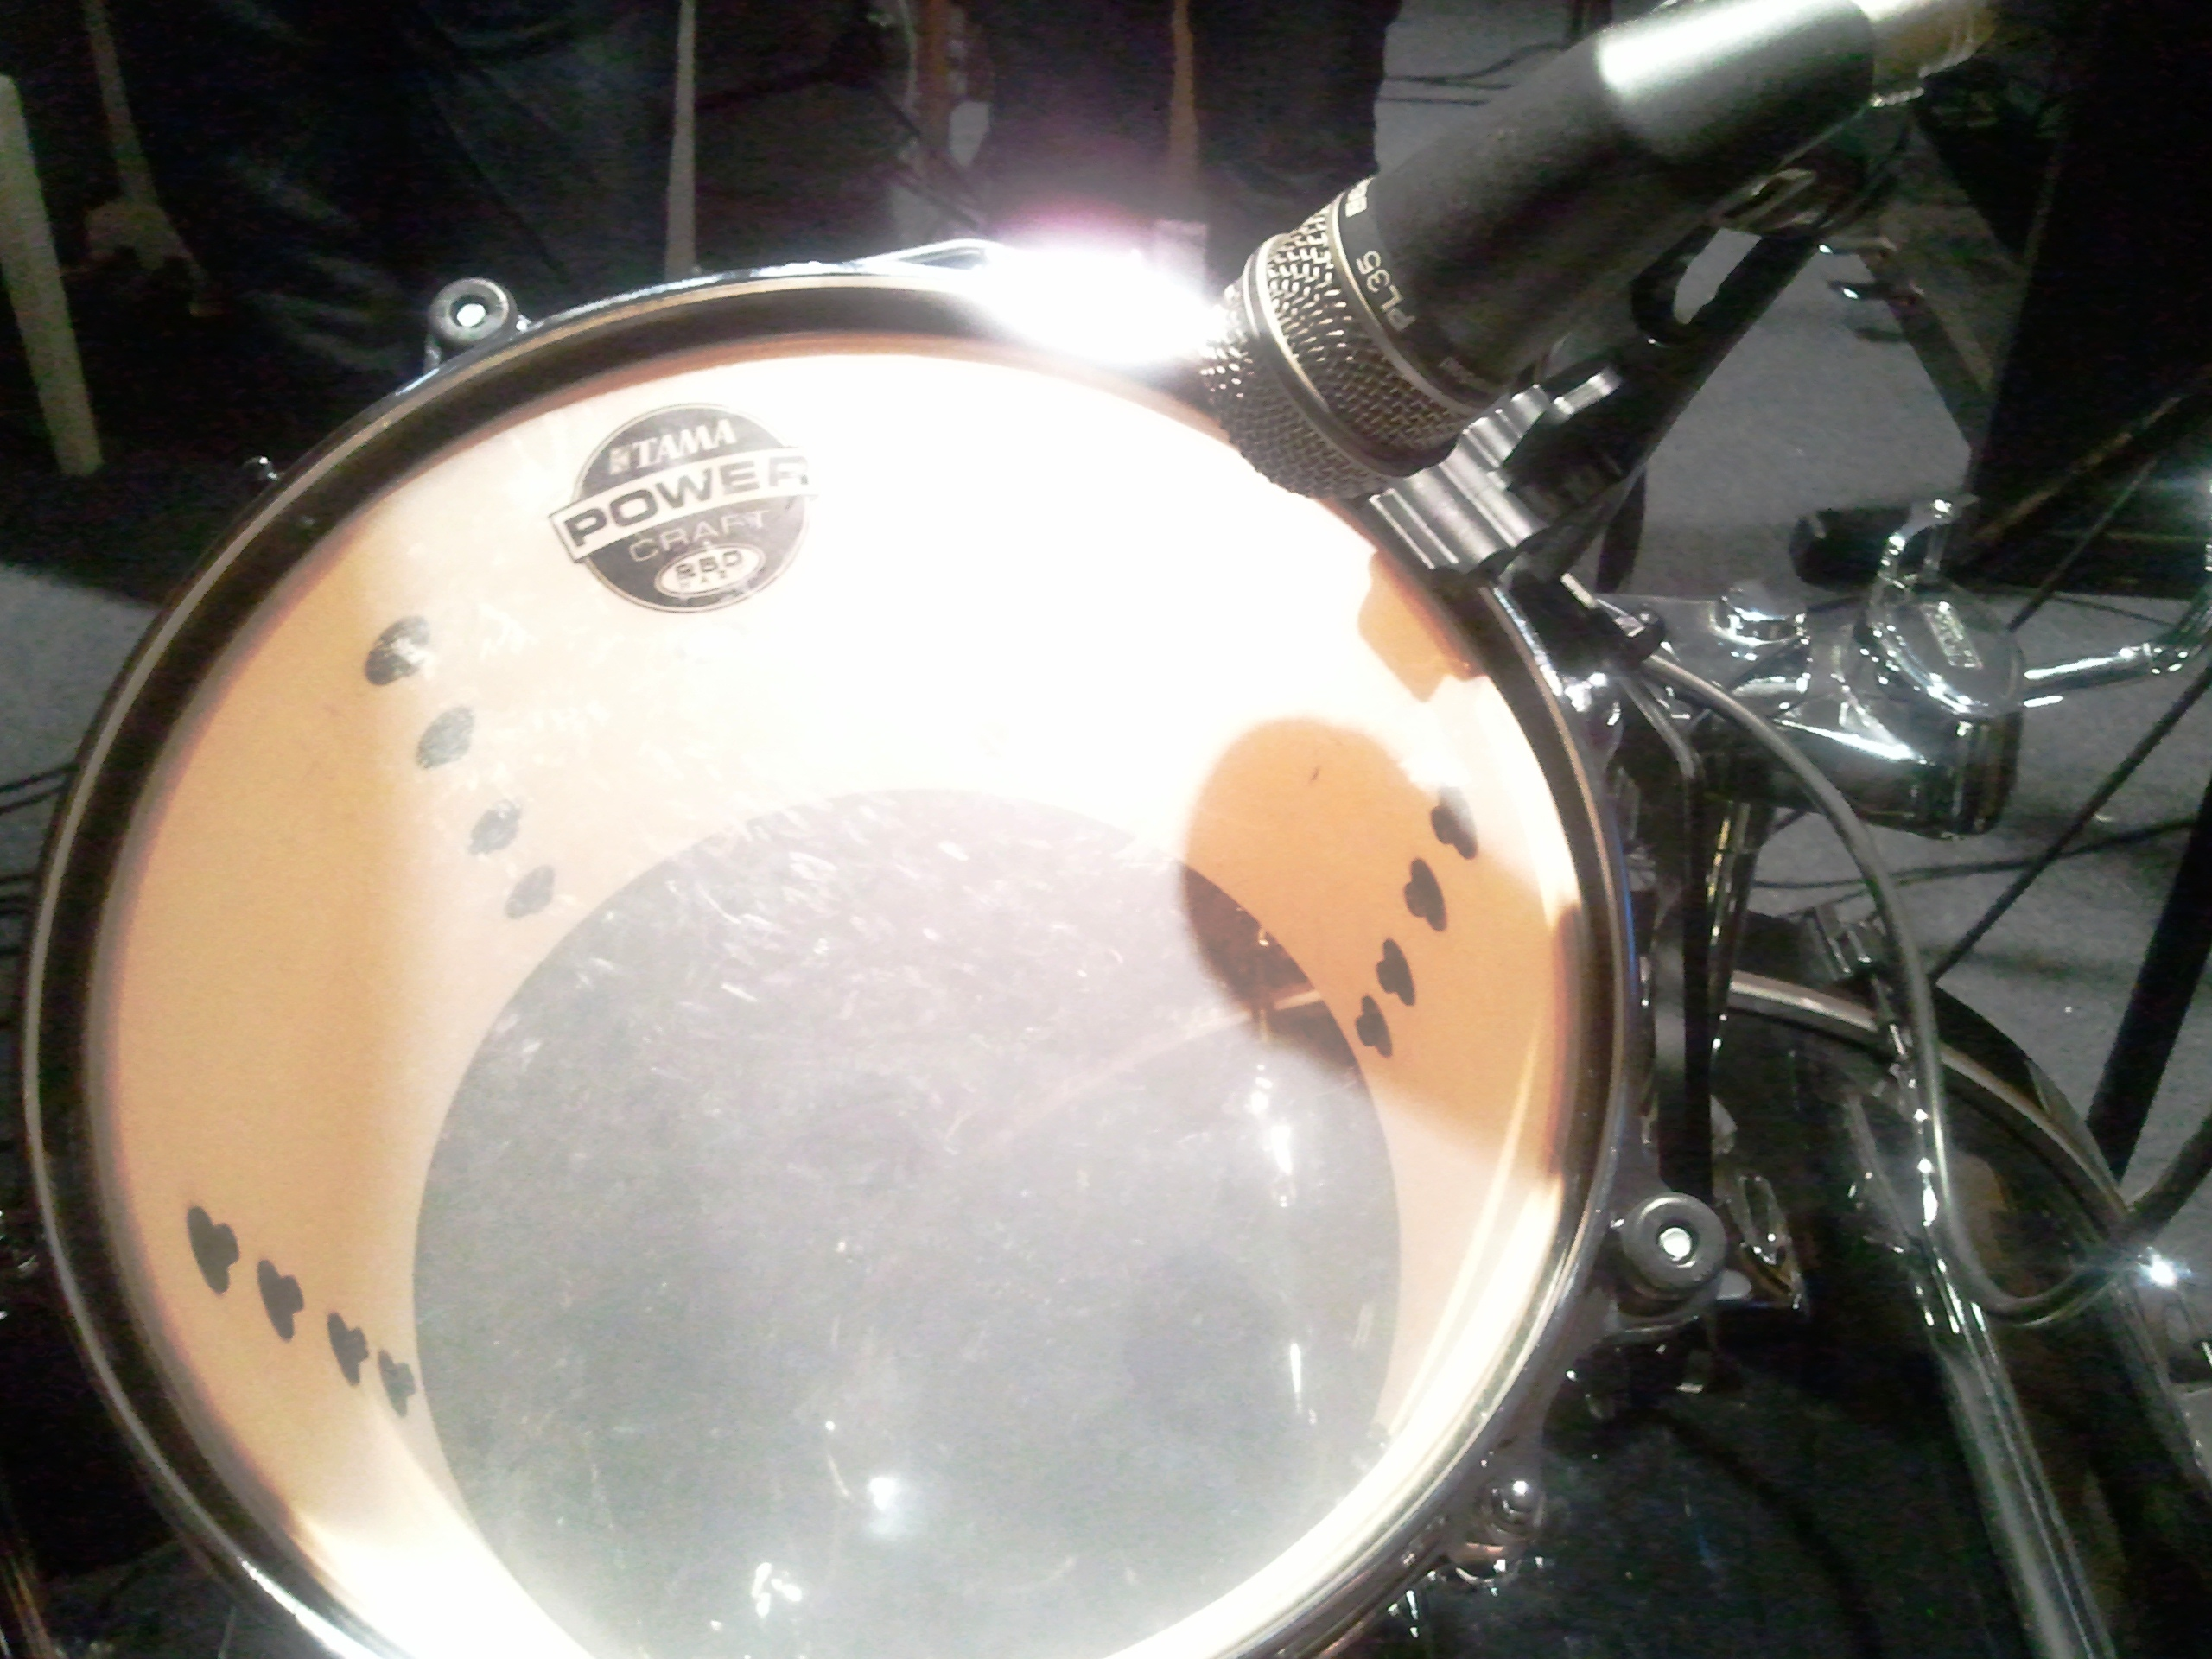
\includegraphics[width=0.8\textwidth]{drums} 
                % Bilddatei aus dem Unterverzeichnis bilder holen, skalieren auf 0.8*Satzspiegel
                \caption{Abnahme einer Trommel mit speziellem Anklemm-Mikrofon}\label{trommelmik}
                \end{figure}
            %------------- BILD ENDE ---------------
    
            %----------- BILD ANFANG -------------
            \begin{figure}[htp]     % h=here, t=top, b=bottom, p=page
                \centering
                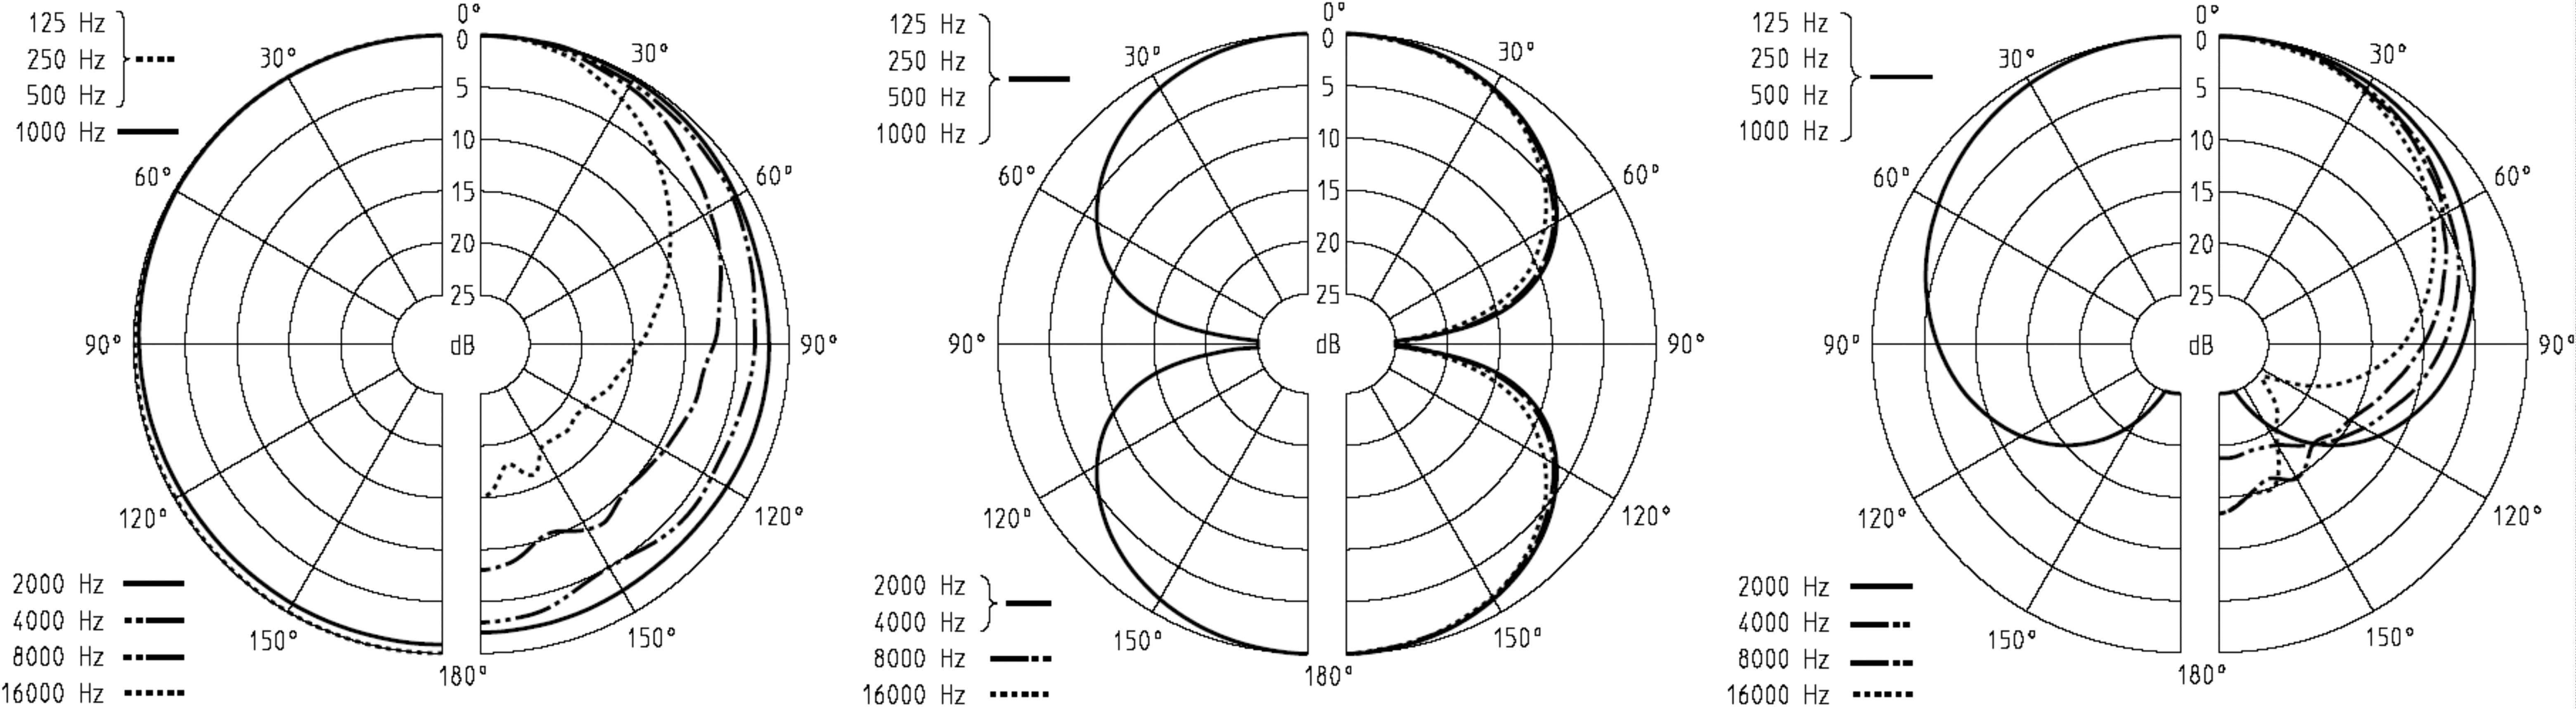
\includegraphics[width=1.0\textwidth]{3x_richtchars}
                \caption[Richtcharakteristiken von Kleinmembran-Studiomikrofonen]{Richtcharakteristiken von Kleinmembran-Studiomikrofonen. V.l.n.r.: Kugel, Acht, Niere. Die Bildbreite ist hier skaliert auf die volle Breite des Satzspiegels.}\label{richtch}
                % bei langen Bildunterschriften kann der optionale Parameter des caption-Befehls so wie hier fxr die Kurzfassung im Abbildungsverzeichnis genutzt werden  
                \end{figure}
            %------------- BILD ENDE ---------------  

        \section{Unterkapitel mit Mathematik, Bildern und Querverweisen}

            Für Formelsatz stellt \LaTeX\ die nummerierte Umgebung equation und die nicht-nummerierte Umgebung displaymath zur Verfügung. Mit label und ref kann dann im Text Bezug auf die Gleichungen genommen werden (Gleichung \ref{gl_fourier}). 

            \begin{equation}\label{gl_fourier}
            S(f) = \int_{-\infty}^{\infty} s(t)e^{-j 2 \pi f t}dt
            \end{equation}

            Mathematik im Zeilenmodus sieht so aus $f_0 = \frac{1}{2\pi} \sqrt{\frac{s}{m}}$, wxhrend dieselbe Gleichung als abgesetzte Formel -- hier mit der displaymath-Umgebung -- so aussieht: 

            \begin{displaymath}
            f_0 = \frac{1}{2\pi} \sqrt{\frac{s}{m}} 
            \end{displaymath}

            Fxr mehrzeilige Herleitungen oder Berechnungen benutzt man in \LaTeX\ die Umgebung eqnarray.

            Einheiten innerhalb von Formeln werden -- wie auch Text -- grundsxtzlich steil (nicht-kursiv) gesetzt. Innerhalb der mathematischen Umgebung nimmt man dafxr eine mbox (make box); die Abstxnde werden mit Komma, Semikolon oder quad eingestellt:

            \begin{displaymath}
            f_0 = \frac{1}{2\pi} \sqrt{\frac{s}{m}} \quad \mbox{[Hz]}
            % \, kleiner Abstand \; mittlerer Abstand \quad groxer Abstand
            \end{displaymath}

            Gleiches gilt fxr Funktionsnamen (sin, cos, arctan, log, ...). Fxr die meisten Funktionsnamen gibt es aber zur Vereinfachung entsprechende Befehle, sodass man nicht immer die mbox braucht.


        \section{Unterkapitel mit zwei Zitaten}

            Das wxrtliche Zitat wird durch Kursivschrift und Anfxhrungszeichen kenntlich gemacht, und natxrlich kommt ein Quellenverweis dazu:

            % \emph = Texthervorhebung durch Schriftumschaltung (emphasize), \medskip: vertikaler Abstand (\smallskip, \bigskip)
            \medskip
            \emph{Nisi irure excepteur eiusmod reprehenderit commodo ipsum exercitation.}
            \medskip

            Alternativ kann man ein Zitat auch in den laufenden Text einflechten, denn wie schon Sowodniok bemerkte, muss sich 
            \emph{Laboris tempor pariatur cillum sunt veniam labore duis ipsum eu cupidatat enim id.}
            Die Quellenverweise werden weiter unten erklxrt.


    \chapter{Ein anderes Kapitel}
                
        \section{Unterkapitel mit Fuxnote, Aufzxhlungen und Tabellen}\label{sec_fussnot}
                
            Fuxnoten sollte man sparsam und bewusst verwenden, erklxrende Zusxtze und Quellenverweise mxglichst in den Text integrieren. Damit bleiben Fuxnoten v.A. reserviert fxr wenige Ergxnzungen, die den Lesefluss stxren wxrden, aber nicht weggelassen werden sollen\footnote{Und so sieht die Fuxnote dann aus}.

            Fxr Aufzxhlungen stellt \LaTeX\ die beiden Umgebungen itemize und enumerate zur Verfxgung. So sieht eine itemize-Aufzxhlung aus:

            \begin{itemize}\setlength{\itemsep}{0ex} % itemsep ist der Abstand zwischen den Punkten der Aufzxhlung
                \item erster Punkt
                \item zweiter Punkt
            \end{itemize}

            Und das ist eine enumerate-Aufzxhlung:

            \begin{enumerate}\setlength{\itemsep}{0ex}
                \item erster Punkt
                \item zweiter Punkt
            \end{enumerate}

            Aufzxhlungen kxnnen auch verschachtelt werden. Als Beispiel dient hier eine enumerate-Umgebung innerhalb einer enumerate-Umgebung:

            \begin{enumerate}\setlength{\itemsep}{0ex}
                \item erster Punkt
                \item 
                    \begin{enumerate}\setlength{\itemsep}{-0.5ex}
                    \item erster Unterpunkt im zweiten Punkt
                    \item zweiter Unterpunkt im zweiten Punkt
                    \item dritter Unterpunkt im zweiten Punkt
                    \end{enumerate}
                \item dritter Punkt
            \end{enumerate}

            Als nxchstes folgt ein Beispiel fxr eine einfache Tabelle. Wie auch die Bilder mxssen die Tabellen stets Unterschrift und Nummer und zwingend einen Verweis im Text haben. In \LaTeX\ wird das wie bei den Abbildungen durch den caption-Befehl und das Befehlspaar label und ref gelxst (Tabelle \ref{t_buli}). Fxr ein modernes Tabellenlayout wird das \LaTeX-booktabs-Paket benutzt (siehe dazu die Kommentare im Quelltext). Die mittlere Spalte ist hier auf feste Breite (6 cm) gesetzt, damit bei viel Text ein automatischer Umbruch erfolgen kann.

            %----------- TABELLE START -------------
            \begin{table}[htp] 
                \centering
                \begin{tabular}{r|p{6cm}|c|c}  % Spalten nach Ausrichtung: l, c, r, p{breite}, mit zwei vertikalen Spaltentrennern
                    %bitte nicht das kleine L "l" und den Vertikalstrich "|" verwechseln!!! :)
                    % kleines L steht fxr eine linksbxndige Spalte, Vertikalstrich erzeugt eine Trennlinie zwischen zwei Spalten
                    \toprule
                    \multicolumn{4}{c}{\large\bfseries Erste Bundesliga, Spielzeit 2011/2012}\\ \midrule
                        Platz & Verein & TD & Punkte\\ \midrule
                        1 & Borussia Dortmund & +20 & 29\\ \midrule
                        2 & Borussia Mxnchengladbach & +14 & 29\\ \midrule
                        3 & FC Bayern Mxnchen & +26 & 28\\ \midrule
                        10 & Hertha BSC Berlin (Ballsportclub), Verein aus der Hauptstadt & $-$1 & 18 \\
                    \bottomrule
                \end{tabular}
                \caption{Bundesligatabelle vom 14. Spieltag}\label{t_buli}
            \end{table}
            %--------- TABELLE ENDE ---------------

            Tabelle \ref{t_buli2} zeigt eine Variante die ein kompakteres und eleganteres Ergebnis liefert, ohne vertikale Striche, dafxr mit eingefxrbten Zeilen.

            %----------- TABELLE START -------------
            \begin{table}[htp] 
                \rowcolors{1}{}{lgray} % bei jeder Zeile die Farbe wechseln, abwechselnd nix und hellgrau
                \centering
                \begin{tabular}{rlcc}  % Spalten nach Ausrichtung: l, c, r, p{breite} 
                    \toprule
                    \multicolumn{4}{c}{\large\sffamily Erste Bundesliga, Spielzeit 2011/2012}\\ \midrule
                        1 & Borussia Dortmund & +20 & 29\\ 
                        2 & Borussia Mxnchengladbach & +14 & 29\\
                        3 & FC Bayern Mxnchen & +26 & 28\\
                        10 & Hertha BSC Berlin & $-$1 & 18 \\ \bottomrule
                \end{tabular}
                \caption{Noch eine Bundesligatabelle vom 14. Spieltag}\label{t_buli2}
            \end{table}
            %--------- TABELLE ENDE ---------------

        \section{Unterkapitel mit drei exemplarischen Quellenverweisen}

            Quellenverweise werden mit Autorennamen und Jahr in runden Klammern gesetzt. Dazu wird hier das \LaTeX-natbib-Paket genutzt; der citep-Befehl erzeugt die Quellenangabe auf Basis der Eintrxge im Literaturverzeichnis. Auf gleiche Weise lassen sich auch mehrere Quellen zusammenfassen

            Auf Bxcher oder andere umfangreichere Quellen soll mit Seitenangabe verwiesen werden. Dafxr stellt der Befehle citep  einen optionalen Parameter zur Verfxgung. Und so sieht dann die vollstxndige Quellenangabe aus

            Die Quellen sollen im Literaturverzeichnis alphabetisch sortiert sein.


            \subsection{Unter-Unterkapitel zu Hyperlinks und Internetquellen}

                Die Beispiele unten im Literaturverzeichnis zeigen exemplarisch, welche Angaben zu den Quellen erforderlich sind (siehe dazu auch die Kommentare im \LaTeX-Quelltext). 

                Und noch eine \LaTeX-Spezialitxt zum Schluss: Durch die Einbindung von url- und hyperref-Paket im header werden die Quellenverweise im PDF-Dokument automatisch mit der jeweiligen Quelle im Literaturverzeichnis verlinkt, und bei Internetquellen werden die URLs anklickbar. Zudem werden die Verzeichnisse (Inhaltsverzeichnis, Abbildungs- und Tabellenverzeichnis) mit den jeweiligen Objekten verlinkt, und es werden Links zwischen jedem \emph{label} und  dazugehxrigem \emph{ref} erzeugt, also z.B. zwischen Bildverweis im Text und dem Bild. Die Farben der Links kxnnen im header frei eingestellt werden. Im hier vorgeschlagenen Layout sind die URLs und die Quellenverweise Dunkelblau, die anderen Links sind nicht hervorgehoben (Schwarz). 


    \chapter{Ergebnisse}

        Der thematische Teil schliext mit einer klaren inhaltlichen, auf der Grundidee aufbauenden thematischen Zusammenfassung, insbesondere bezogen auf die in der Arbeit gewonnenen eigenen Erkenntnisse und deren mxgliche Auswirkungen auf Forschung und Wissenschaft. 

        Ganz am Schluss, nach eventuellen Anhxngen, nach Abbildungs- und evtl. Tabellenverzeichnis, und nach dem Literaturverzeichnis, folgt die Eigenstxndigkeitserklxrung, die unterschrieben werden muss.